%%%%%%%%%%%%%%%%%%%%%%%%%%%%%%%%%%%%%%%%%%%%%%%%%%%%%%%%%%%%%%%%%%%%%%%%%%%%%%%%%%%%%%%%%%
%%
%% Description:		This is an example presentation using the beamerthemedhbw
%%
%%					The beamerthemedhbw is based on jacksbeamertheme
%%					(https://github.com/JacknJo/jacksbeamertheme)
%%
%% Author:			Hannes Bartle																				
%% 					DHBW Ravensburg Campus Friedrichshafen		
%%					September 2016	
%% 
%% The beamerthemedhbw is free software: you can redistribute it and/or modify
%% it under the terms of the GNU General Public License as published by
%% the Free Software Foundation, either version 3 of the License, or
%% (at your option) any later version.
%% 
%% The beamerthemedhbw is distributed in the hope that it will be useful,
%% but WITHOUT ANY WARRANTY; without even the implied warranty of
%% MERCHANTABILITY or FITNESS FOR A PARTICULAR PURPOSE.  See the
%% GNU General Public License for more details.
%% 
%% You should have received a copy of the GNU General Public License
%% along with the beamerthemedhbw.  If not, see <http://www.gnu.org/licenses/>.
%% 
%% 
%%%%%%%%%%%%%%%%%%%%%%%%%%%%%%%%%%%%%%%%%%%%%%%%%%%%%%%%%%%%%%%%%%%%%%%%%%%%%%%%%%%%%%%%%%


\documentclass[	12pt, 				
				t,					
				aspectratio=169,
				%handout-PLACEHOLDER
				]{beamer}

\usepackage{dhbwstyle}

\title{Algorithmen II}

\begin{document}
	
	\begin{frame}[noframenumbering]
		\titlepage
	\end{frame}

	\begin{frame}{Outline}
		\tableofcontents
	\end{frame}

    \outlineFrame{Arten von Algorithmen}
    \outlineSubframe{Backtracking}
\begin{frame}{Allgemeines}{Eigenschaften}
    \begin{itemize}
        \item Grundlegende Algorithmenstrategie
        \item Findet theoretisch:
        \begin{itemize}
        \item alle Lösungen für ein gegebenes Problem...
        \item ...in einer endlichen Zeit
        \end{itemize}
        \item Nutzt das \textbf{trial and error} Prinzip
    \end{itemize}
\end{frame}

\begin{frame}{Methodik}
    \begin{itemize}
        \item Sind rekursiv implementiert
        \item Es werden inkrementell Teillösungen "`ausprobiert"'
        \item Wird eine Teillösung als ungeeignet erkannt, wird diese verworfen
        \item Implikationen daraus:
        \begin{itemize}
            \item Problem muss ein Kriterium für Nicht-Erfüllbarkeit liefern
            \item Oder anders: Die Lösung muss bestimmte Bedingungen erfüllen
            \item Man spricht in der Regel von \textbf{Constraint-Satisfaction-Problems}
        \end{itemize}
        \item Visualisieren lässt sich das z.B. als Entscheidungsbaum
    \end{itemize}
\end{frame}

\begin{frame}{Entscheidungsbaum}{Backtracking Algorithmen}
    \begin{figure}
    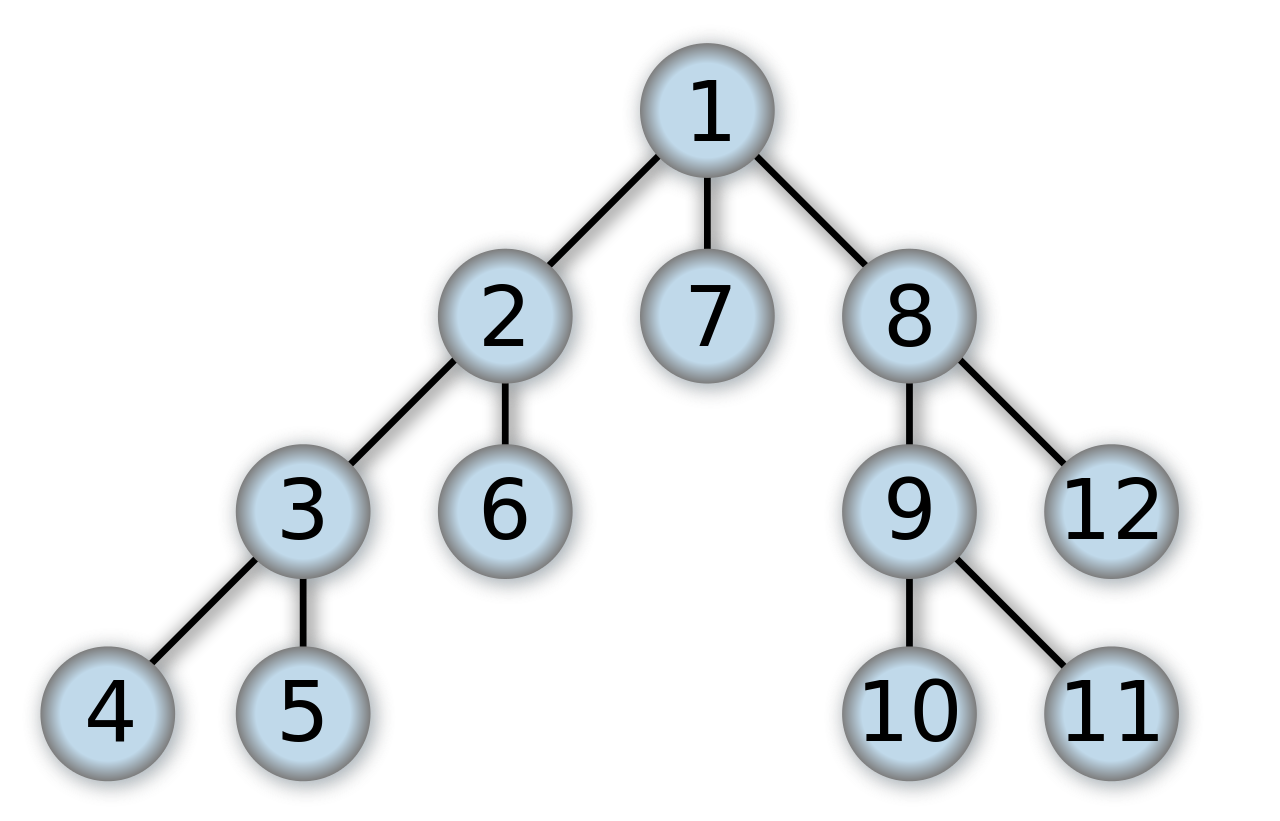
\includegraphics[height=5cm]{graph/backtracking_tree}
    \caption*{Quelle: \cite{wiki:backtr}}
    \end{figure}
\end{frame}

\begin{frame}{Vor- und Nachteile}
    \begin{itemize}
        \item Es werden alle (sinnvollen) Lösungen ausprobiert
        \item Umgekehrt kann definitiv ausgesagt werden, dass keine Lösung existiert, wenn Sie nicht über Backtracking gefunden werden kann
        \item Jedoch sehr ineffizient
        \begin{itemize}
            \item Komplexität im Worst Case ist $O(z^n)$ (Wobei $z$ der Verzweigungsgrad ist)
            \item Somit ergibt sich für alle $z>1$ eine exponentielle Laufzeit
            \item Daher eher für Probleme mit kleinem Lösungsbaum geeignet
        \end{itemize}
    \end{itemize}
\end{frame}

\begin{frame}[allowframebreaks]{Anwendungen}{Von Backtracking (Vgl. \cite{wiki:backtracking})}
    \begin{itemize}
        \item \textbf{Damenproblem}
        \begin{itemize}
            \item Auf einem $n\times n$ Schachfeld sollen $n$ Damen so platziert werden, dass sie sich nicht gegenseitig schlagen können
        \end{itemize}
        \item \textbf{Springerproblem}
        \begin{itemize}
            \item Auf einem $M\times N$ Schachfeld soll ein Springer einen Weg finden, durch den jedes Feld \textbf{genau einmal} besucht wird.
        \end{itemize}
        \item \textbf{Sudoku}
        \item \textbf{Färbeproblem}
        \begin{itemize}
            \item Eine Landkarte mit $B$ Ländern soll mit $N$ verschiedenen Farben eingefärbt werden
            \item Gesucht wird eine Einfärbung, bei der angrenzende Länder immer verschiedene Farben haben
        \end{itemize}
        \item \textbf{Wegsuche in Graphen}
        \begin{itemize}
            \item Hierzu gehört zum Beispiel auch das finden eines Weges in einem Labyrinth
        \end{itemize}
        \item Viele Backtracking Probleme sind \textbf{NP-vollständig}
    \end{itemize}
\end{frame}
    \outlineSubframe{Divide and Conquer}
\begin{frame}{Motivation}
    \begin{itemize}
        \item Das Lösen großer Probleme fällt oft schwer
        \begin{itemize}
            \item Sowohl für Menschen
            \item Als auch Computer
        \end{itemize}
        \item Meist ist es einfacher, das Problem in Teilprobleme zu unterteilen
        \item ...und diese separat voneinander zu lösen
        \item Wir machen dies oft ganz automatisch
        \item Bei Algorithmen spricht man hierbei vom \textbf{Divide and Conquer} Verfahren
    \end{itemize}
\end{frame}

\begin{frame}{Simples Beispiel}{Multiplikation}
    $$a\cdot b = \overbrace{b+b+\cdots+b}^{a\text{ mal}}$$
    
    $$a\cdot b = \overbrace{(b+b+\cdots+b)}^{\frac{a}{2}\text{mal}} + \overbrace{(b+b+\cdots+b)}^{\frac{a}{2}\text{mal}} $$
    
    $$a\cdot b = 2\cdot \overbrace{(b+b+\cdots+b)}^{\frac{a}{2}\text{mal}}$$
\end{frame}

\begin{frame}{Grundsätze}{Des Divide and Conquer Verfahrens}
    \begin{itemize}
        \item Ein gegebenes Problem wird aufgeteilt...
        \item ...in zwei (oder mehr) kleinere Teilprobleme
        \item Dies geschieht rekursiv solange...
        \item ...bis sich die Teilprobleme trivial direkt lösen lassen
        \item Am Ende werden die Teilergebnisse zur Gesamtlösung zusammengefügt
        \item Es gibt ein ähnliches Vorgehen, bei dem man das Problem lediglich auf \textit{ein} kleineres Teilproblem reduziert
        \begin{itemize}
            \item Dies nennt man auch \textbf{Decrease and Conquer}
        \end{itemize}
    \end{itemize}
\end{frame}

\begin{frame}{Vorteile}{Von D\&C Algorithmen (Vgl. \cite{wiki:dac})}
    \begin{itemize}
        \item \textbf{Starke Lösungsstrategie}
        \begin{itemize}
            \item Hilft dabei, Lösungen für komplexe Probleme zu finden
            \item Solange man einen Weg findet, das Problem in kleinere Subprobleme zu teilen
        \end{itemize}
        \item \textbf{Algorithmeneffizienz}
        \begin{itemize}
            \item Der D\&C Ansatz hat oft effizientere Algorithmen für bekannte Probleme gefunden
            \item Zum Beispiel: Quicksort, Mergesort und FFT
            \item Wenn sich ein Problem der Größe $n$ immer in $p$ Teilprobleme der Größe $~\frac{n}{p}$ teilen lässt, so ist die Komplexität von $O(n\log_p n)$
        \end{itemize}
    \end{itemize}
\end{frame}

\begin{frame}{Vorteile}{Von D\&C Algorithmen (Vgl. \cite{wiki:dac})}
    \begin{itemize}
        \item \textbf{Parallelisierung}
        \begin{itemize}
            \item Teilprobleme können oft parallel bearbeitet werden
            \item Dadurch teils erhebliche Zeitersparnis
        \end{itemize}
        \item \textbf{Speicherzugriff}
        \begin{itemize}
            \item D\&C Algorithmen können den Speicher meist effizienter (=schneller) nutzen
            \item Wenn die Teilprobleme klein genug sind können diese ggf. direkt im Prozessorcache berechnet werden
            \item Dieser ist im Vergleich zum RAM deutlich schneller durch höhere Taktraten und physische Nähe
        \end{itemize}
    \end{itemize}
\end{frame}

\begin{frame}{Herausforderungen}{Bei der Implementierung von D\&C Algorithmen (Vgl. \cite{wiki:dac})}
\begin{itemize}
    \item \textbf{Rekursion}
    \begin{itemize}
        \item Implementierung erfolgt in der Regel über rekursive Aufrufe
        \item Dies ist häufig komplexer in der Implementierung und dem Verständnis
    \end{itemize}
    \item \textbf{Aufruftiefe}
    \begin{itemize}
        \item Je nachdem wie oft der rekursive Aufruf erfolgt führt das zu Problemen
        \item Je nach Sprache und Compiler ist ggf. nur eine Rekursionstiefe möglich
        \item Dies kommt durch die ggf. beschränkte Größe des \textit{Call Stacks}
        \item Bei zu tiefer Rekursion kann es so zum \textit{Stack Overflow} kommen
    \end{itemize}
\end{itemize}
\end{frame}

\begin{frame}{Herausforderungen}{Bei der Implementierung von D\&C Algorithmen (Vgl. \cite{wiki:dac})}
    \begin{itemize}
        \item \textbf{Auswahl des "`trivialen Problems"'}
        \begin{itemize}
            \item Die Auswahl des direkt lösbaren Teilproblems ist nicht immer direkt ersichtlich
            \item In einigen Fällen ist ein Teilen bis zum kleinstmöglichen Teilproblem nicht sinnvoll
            \item Und effizienter ist es ein größeres Teilproblem direkt zu lösen
            \item Beispiel: Determinantenberechnung in Matrizen
        \end{itemize}
    \end{itemize}
\end{frame}
    
    %\outlineFrame{Suchalgorithmen}
    %\begin{frame}{Suchalgorithmen}{Motivation}
    \begin{itemize}
        \item Dienen dazu mit großen Datenmengen zu arbeiten
        \item Um bestimmte Informationen zu finden
        \item Beispiele (Digital und analog):
        \begin{itemize}
            \item Finden einer Übersetzung im Wörterbuch 
            \item Finden von Websites
            \item Suchen von bestimmten Buchabschnitten nach Thema (über Inhaltsverzeichnis oder Index)
        \end{itemize}
    \end{itemize}
\end{frame}

\begin{frame}{Allgemeine Aspekte}{Der Suche}
    \begin{itemize}
        \item Oft wird nach den \textit{Werten} für bestimmte \textit{Schlüssel} gesucht
        \item Die Suche in einer beliebigen Sammlung von Daten ist in der Regel nur schwer optimierbar
        \begin{itemize}
            \item Man muss jedes Element der Sammlung einzeln betrachten um ein bestimmtes Element zu finden
            \item Komplexität: $O(N)$
        \end{itemize}
        \item Aus diesen Gründen werden zum suchen teils spezielle Datenstrukturen verwendet:
        \begin{itemize}
            \item Symboltabellen
            \item Hashtables
            \item Suchbäume
        \end{itemize}
    \end{itemize}
\end{frame}

\begin{frame}{Allgemeine Aspekte}{Der Suche}
    \begin{itemize}
        \item Gemeinsamkeit der Suchstrukturen:
        \begin{itemize}
            \item Sind meist nach einem bestimmten Kriterium sortiert
        \end{itemize}
        \item Dadurch lassen sich die Strukturen deutlich einfacher durchsuchen
        \item Stichwort: \textbf{Binärsuche}
    \end{itemize}
\end{frame}
    
    \outlineFrame{Sortieralgorithmen}
    \outlineSubframe{Insertion Sort}
    \begin{frame}{Insertion Sort}{Grundprinzip (Siehe \cite{ottmann2017} S. 85ff)}
    \begin{itemize}
        \item Gegeben sein eine Liste mit $N$ Elementen
        \item Jedes Element wird nacheinander betrachtet
        \item Und an der korrekten Stelle der bereits betrachteten Elemente eingefügt
        \item Dadurch ergibt sich:
        \begin{itemize}
            \item Eine bereits sortierte Teilliste
            \item Eine Restliste mit den noch einzusortierenden Elementen
        \end{itemize}
    \end{itemize}
\end{frame}

\begin{frame}{Insertion Sort}{Praktisches Beispiel}
\end{frame}

\begin{frame}{Vor- und Nachteile (Siehe \cite{ottmann2017} S. 85ff)}
    \begin{itemize}
        \item Implementierung ist relativ simpel
        \item Jedoch viele Vergleiche und ggf. Verschiebungen nötig
        \item Komplexität beträgt hierfür $O(N^2)$
    \end{itemize}
\end{frame}


    
    \outlineSubframe{Bubble Sort}
    \begin{frame}{Bubble Sort}{Grundprinzip (Siehe \cite{ottmann2017} S. 89ff)}
    \begin{itemize}
        \item Eine Liste wird Elementweise betrachtet
        \item Jedes Element wird mit seinem Nachfolger verglichen
        \item Ist der Nachfolger kleiner, so werden die Elemente getauscht
        \item Dies wird solange wiederholt, bis die komplette Liste durchlaufen wurde ohne, dass eine Vertauschung durchgeführt wurde
        \item Der Name "`Bubble"' leitet sich davon ab, dass die größten Element sich am oberen Ende der Liste wie eine "`Blase"' sammeln
    \end{itemize}
\end{frame}

\begin{frame}{Insertion Sort}{Praktisches Beispiel}
\end{frame}

\begin{frame}{Vor- und Nachteile}{Siehe \cite{ottmann2017} S. 89ff}
    \begin{itemize}
        \item Wohl mit der simpelste Algorithmus
        \item Jedoch ineffizient $\rightarrow$ Komplexität $O(N^2)$
        \item Auch wenn z.B. Insertion Sort die gleiche Komplexität hat ist dieser in der Regel deutlich schneller
        \item Daher nur wenige sinnvolle praktische Anwendungen:
        \begin{itemize}
            \item Beispielsweise erkennen (und korrigieren) von sehr kleinen Fehlern in "`beinahe sortierten"' Arrays (Anwendung in der Computergrafik)
        \end{itemize}
    \end{itemize}
\end{frame}
    
    \outlineSubframe{Selection Sort}
    \begin{frame}{Selection Sort}{Grundprinzip (Vgl. \cite{ottmann2017} S. 82f, \cite{wayne2014}, S. 272f)}
    \begin{itemize}
        \item Gegeben ist eine Liste mit Elementindizes $1$ bis $N$
        \item Beginnend mit $M=1$ führe folgende Schritte durch:
        \begin{itemize}
            \item Suche das Minimum der Liste im Bereich $M\ldots N$
            \item Tausche das Minimum mit dem Element an der Stelle $M$
            \item Wiederhole diesen Vorgang für die Teilliste von $M+1\ldots N$ (Solange bis $M=N$)
        \end{itemize}
    \end{itemize}
\end{frame}
    
    \outlineSubframe{Heapsort}
    \begin{frame}{Heapsort}{Grundprinzip (Vgl. \cite{fahr:algo}, S. 12ff)}
    \begin{itemize}
        \item Sortiert nicht direkt Listen sondern nur die spezielle Struktur "`Heap"'
        \item Das heißt die Daten müssen entweder in dieser Form vorliegen
        \item ...Oder erst in diese Struktur umgewandelt werden
        \item Heap kann als Binärbaum interpretiert werden
        \item Heapsort besteht aus dem wiederholten Entfernen der Wurzel...
        \item ...Und dem nachfolgenden "`versickern"' der restlichen Element
    \end{itemize}
\end{frame}

\begin{frame}{Heap}{Definition}
    \begin{alertblock}{Heap (Definition als Liste, Vgl. \cite{fahr:algo}, S. 12ff)}
    Eine Folge $F = k_1, k_2, \ldots,k_n$ von $n$ Schlüsseln nennen wir dann Heap, wenn
    $$k_i\le k_{\frac{i}{2}}$$
    \end{alertblock}
\end{frame}

\begin{frame}{Heap}{Definition (Vgl. \cite{fahr:algo}, S. 12ff)}
    \begin{alertblock}{Heap (Binärbaum)}
    Ein Heap ist ein vollständiger Binärbaum, in dem der Schlüssel jedes Knotens mindestens so groß ist wie der Schlüssel seiner Söhne
    \end{alertblock}
\end{frame}

\begin{frame}{Heapsort}{Sortieren (Vgl. \cite{fahr:algo}, S. 12ff)}
\begin{alertblock}{Vorgehen Sortieren}
\begin{itemize}
    \item Gebe den Wurzelknoten des Baumes aus und entferne diesen
    \item Setze das letzte Element im Baum an die Wurzel
    \item Versickere die neue Wurzel im Baum
    \item Wiederhole den Prozess bis der Baum leer ist
\end{itemize}
\end{alertblock}
\end{frame}

\begin{frame}{Heapsort}{Versickern (Vgl. \cite{fahr:algo}, S. 12ff)}
\begin{alertblock}{Vorgehen Versickern}
\begin{itemize}
    \item Vergleiche den Wurzelknoten mit dem größten Kindknoten
    \item Ist der Wurzelknoten kleiner als der größte Kindknoten:
    \begin{itemize}
        \item Vertausche den Kindknoten mit dem Wurzelknoten
        \item Wiederhole dies bis beide Kindknoten kleiner als der Wurzelknoten sind (Bzw. keine Kindknoten mehr vorhanden sind)
    \end{itemize}
\end{itemize}
\end{alertblock}
\end{frame}
    
    \outlineSubframe{Quicksort}
    \begin{frame}{Quicksort}{Grundprinzipien (Vgl. \cite{ottmann2017} S. 93ff, \cite{wayne2014} S. 313-330)}
    \begin{itemize}
        \item Basiert auf dem \textbf{Divide and Conquer} Prinzip
        \item Es wird ein Vergleichselement $x$ gewählt
        \item Und die Liste in eine linke und rechte Teilliste gliedert
        \begin{itemize}
            \item Linke Teilliste: Alle Elemente sind kleiner(oder gleich) $x$
            \item Rechte Teilliste: Alle Elemente sind größer(oder gleich) $x$
        \end{itemize}
        \item Führe wieder Quicksort auf den beiden Teillisten aus
    \end{itemize}
\end{frame}

\begin{frame}{Grundlegendes Vorgehen}{Quicksort (Siehe \cite{fahr:algo} S. 8ff)}
    \begin{itemize}
        \item Setze linken Zeiger $i$ auf das erste Element
        \item Setze rechten Zeiger $j$ auf das letzte Element
        \item Solange $i<j$
        \begin{itemize}
            \item Erhöhe $i$ bis $a[i]\ge x$
            \item Verringere $j$ bis $a[j]\le x$
            \item Wenn $i<j$, dann vertausche die Elemente
        \end{itemize}
    \end{itemize}
\end{frame}    
    
    %\outlineSubframe{Slowsort}
    %\begin{frame}{Slowsort}{Ein humoristischer Ansatz an Sortierungen}
    \begin{itemize}
        \item 1986 von Andrei Broder und Jorge Stolfi entwickelt
        \item Teil ihres Papers "`Pessimal Algorithms and Simplexity Analysis"
        \item Ziel war ein möglichst ineffizienten Algorithmus zu schaffen
        \begin{itemize}
            \item Ohne Nutzung von zufälligen Faktoren
            \item ...und ohne "`überflüssige"' Operationen einzubauen
        \end{itemize}
        \item Basiert auf dem \textbf{Multiply and Surrender} (Parodie auf Divide and Conquer) Prinzip
    \end{itemize}
\end{frame}

\begin{frame}{Slowsort}{Ablauf}
    \begin{itemize}
        \item Besteht im Grund aus zwei Schritten:
        \begin{itemize}
            \item 1. Finde das Maximum der Liste und platziere es am Ende
            \item 2. Sortiere die verbleibende Teilliste
        \end{itemize}
        \item Ineffizienz kommt durch die rekursive Umsetzung des ersten Schritts:
        \begin{itemize}
            \item 1.1 Finde (rekursiv) das Maximum der ersten Listenhälfte
            \item 1.2 Finde (rekursiv) das Maximum der zweiten Listenhälfte
            \item 1.3 Vergleiche die Maxima und tausche ggf.
        \end{itemize}
        \item Die untere Grenze der Komplexität lässt sich angeben mit $\Omega (n^{\frac{\log_2(n)}{2+\epsilon}})$
        \item Damit ist selbst der Best-Case schlechter als der Worst-Case von Bubble Sort
    \end{itemize}
\end{frame}
    
    \printbibliographyframe
    
	\section*{Kontakt}
	\begin{frame}{Kontakt}{}
	\begin{itemize}
		\item E-Mail: \href{mailto:lukas.abelt@airbus.com}{lukas.abelt@airbus.com}
		\item GitHub: \url{https://www.github.com/LuAbelt}
		\item GitLab: \url{https://www.gitlab.com/LuAbelt}
		\item Telefon(Firma): 07545 - 8 8895
		\item Telegram: LuAbelt
	\end{itemize}
\end{frame}
	

\end{document}